\chapter{ML with TensorFlow}

Overview

\section{Introduction}

\section{Artificial Neural Networks}

\section{Convolutional Neural Networks}

\section{Recurrent Neural Networks}

\section{Weight Initialization}

\subsection{Activation Functions}

\textcolor{blue}{Activation functions are XXXXXXXX}

\subsubsection{Why Non-linear}

\textcolor{blue}{Non-linear is necessary XXXXXXXXXX}

\subsubsection{Advancements}

\textcolor{green}{TODO: From step function to ?selu}

\subsubsection{Popular Activation Functions}

\textcolor{blue}{Activation functions can be grouped into two main categories -- smooth and not smooth. Smooth activation functions (such as sigmoid) are differentiable at every point along the function where as the other activation functions are not differentiable at every location (relu).}

% history
%differentiable everywhere, monotonic, and smooth.

\textcolor{blue}{linear (see above), }
	
\textcolor{blue}{tanh and sigmoid, (better because non-linear). however would saturate}

\textcolor{blue}{ReLu, better because \textcolor{red}{help prevent saturation}, but still have problems \textcolor{red}{can "die" at 0.} }

\textcolor{blue}{ELU fuctions. they prevent the "dying" problem by being \textcolor{red}{non-zero} but their main drawback is that they are more computationally expensive due to the calculation of the exponent.}

\paragraph{Smooth Non-linear}

\subparagraph{Sigmoid}

\textcolor{blue}{The sigmoid\index{sigmoid} activation function.}

\textcolor{blue}{calibrated probability estimate}


% {{{act_smooth_sigmoid}}}
\begin{figure}
\centering
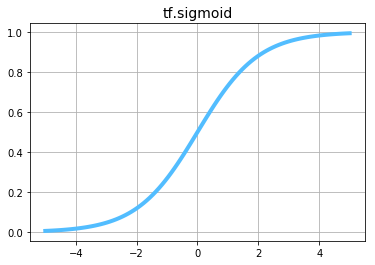
\includegraphics[width=0.65\textwidth]{./sync_imgs/act/smooth/sigmoid.png}
\label{fig:act_smooth_sigmoid}
\end{figure}

% {{{act_smooth_tangent}}}
\begin{figure}
\centering
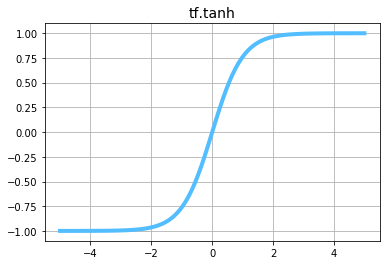
\includegraphics[width=0.65\textwidth]{./sync_imgs/act/smooth/tangent.png}
\label{fig:act_smooth_tangent}
\end{figure}

\subparagraph{ELU}

\textcolor{blue}{\textcolor{red}{CITE}. Smooth, monotonic, and non-zero in the negative portion of the input. The main drawback is that they are more computationally expensive (due to calculating the exponential)}


\begin{equation}
{
	ELU = f(x) = \left\{
	\begin{array}{ll}
	\alpha(e^x - 1) x & \quad $for$ \ x < 0 \\
	x & \quad $for$ \ x \ge 0
	\end{array}
	\right.
}
\label{eq:act_elu_def}
\end{equation}


% {{{act_smooth_elu}}}
\begin{figure}
\centering
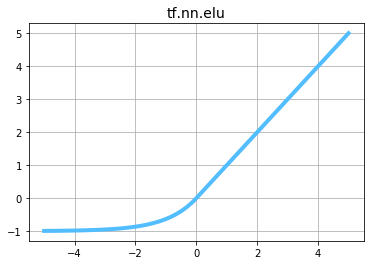
\includegraphics[width=0.65\textwidth]{./sync_imgs/act/smooth/elu.png}
\label{fig:act_smooth_elu}
\end{figure}

% {{{act_smooth_selu}}}
\begin{figure}
\centering
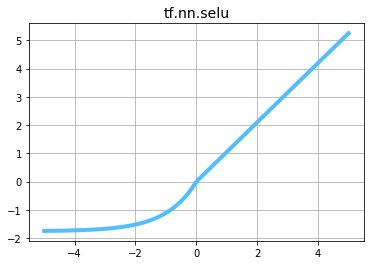
\includegraphics[width=0.65\textwidth]{./sync_imgs/act/smooth/selu.png}
\label{fig:act_smooth_selu}
\end{figure}


\subparagraph{Softplus}

\textcolor{blue}{continuous and differentiable at zero. However, due to the natural log and exponential function, there is added computation compared to th ReLU.}

% typcially discouraged in practice since ReLU achieves similar results and is less computationally expensive

\begin{equation}
{
	Softplus = f(x) = \ln{(1+e^x)}
}
\label{eq:act_softplus_def}
\end{equation}


% {{{act_smooth_softplus}}}
\begin{figure}
\centering
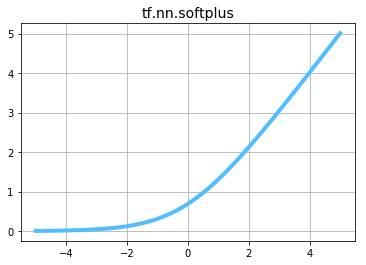
\includegraphics[width=0.65\textwidth]{./sync_imgs/act/smooth/softplus.png}
\label{fig:act_smooth_softplus}
\end{figure}

% {{{act_smooth_softsign}}}
\begin{figure}
\centering
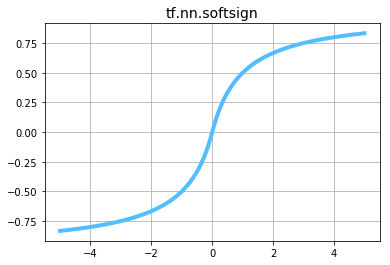
\includegraphics[width=0.65\textwidth]{./sync_imgs/act/smooth/softsign.png}
\label{fig:act_smooth_softsign}
\end{figure}


\paragraph{Not Smooth Non-linear}

\subparagraph{ReLU}

\begin{equation}
{
	ReLU = f(x) = \left\{
	\begin{array}{ll}
	0 & \quad $for$ \ x < 0 \\
	x & \quad $for$ \ x \ge 0
	\end{array}
	\right.
}
\label{eq:act_relu_def}
\end{equation}

% {{{act_notsmooth_relu}}}
\begin{figure}
\centering
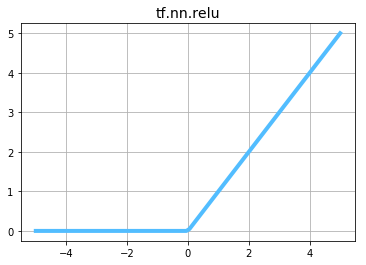
\includegraphics[width=0.65\textwidth]{./sync_imgs/act/notsmooth/relu.png}
\label{fig:act_notsmooth_relu}
\end{figure}

\subparagraph{Leaky ReLU}

\textcolor{blue}{The Leaky ReLU (Eq~\ref{eq:act_leaky_relu_def}) was designed in attempt to address the dying ReLU issue \textcolor{red}{CITE}. Rather than simply outputting a zero in the negative range, the Leaky ReLU will will have a small non-zero slope (user specified) -- allowing weight updating and training to continue.}

\textcolor{green}{TODO: randomized Leaky ReLU \textcolor{red}{cite} --- $\alpha$ (from PReLU) is sampled from a uniform distribution randomly. The net-effect could be considered similar to drop out since, technically, there is a different network for each value of $\alpha$, resulting in an ensemble of sorts. At test time, the values for $\alpha$ are averaged.}

\begin{equ}[!ht]
	\begin{equation}
	{
		Leaky ReLU = f(x) = \left\{
		\begin{array}{ll}
		N x & \quad $for$ \ x < 0 \\
		x & \quad $for$ \ x \ge 0
		\end{array}
		\right.
	}
	\label{eq:act_leaky_relu_def}
	\end{equation}
\caption{where $N$ is a constant. $N$ is typically set to 0.01}
\end{equ}

% {{{act_notsmooth_leakyrelu}}}
\begin{figure}
\centering
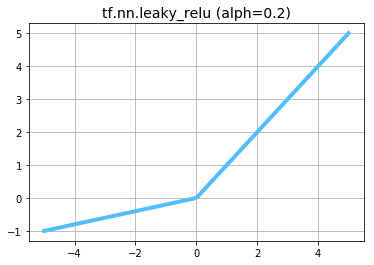
\includegraphics[width=0.65\textwidth]{./sync_imgs/act/notsmooth/leakyrelu.png}
\label{fig:act_notsmooth_leakyrelu}
\end{figure}

\subparagraph{ReLU6}

\textcolor{blue}{In general, this function is referred to as a {ReLUN}\index{ReLUN} function, where $N$ is some constant. However, in practice, $6$, was determined to be the optimal value.\textcolor{red}{CITE}. \textcolor{red}{This capped value, may help learn the sparse values sooner.} By having the upper limit bounded, the prepare the network for a fixed point precision for inference --- if the upper limit is unbounded, then you may loose too many bits to \textcolor{red}{Q} portion of the fixed point number.}
		

\textcolor{blue}{Similar to the ReLU fuction, only the output is capped to six in the positive domain.}

\begin{equation}
{
	ReLU6 = f(x) = min{(max{(0,x)},6)}
}
\label{eq:act_ReLU6_def}
\end{equation}

% {{{act_notsmooth_relu6}}}
\begin{figure}
\centering
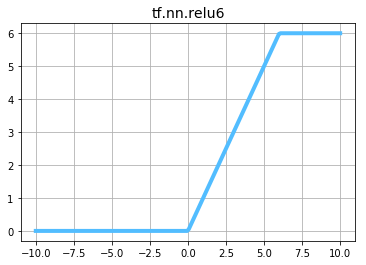
\includegraphics[width=0.65\textwidth]{./sync_imgs/act/notsmooth/relu6.png}
\label{fig:act_notsmooth_relu6}
\end{figure}

\subparagraph{PReLU}

\begin{equ}[!ht]
	\begin{equation}
	{
	PReLU = f(x) = \left\{
		\begin{array}{ll}
			\alpha x & \quad $for$ \ x < 0 \\
			x & \quad $for$ \ x \ge 0
		\end{array}
		\right.
	}
	\label{eq:act_prelu_def}
	\end{equation}
\caption{where $\alpha$ is a parameterized --- a learned parameter from training.}
\end{equ}

\textcolor{blue}{$\alpha$, rather than being hard coded, is determined during training by the data. The logic being that the value would be more optimal than we could set \textcolor{red}{CITE}}

% {{{act_notsmooth_prelu}}}
\begin{figure}
\centering
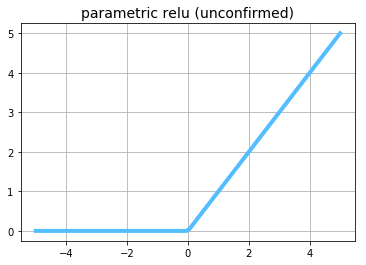
\includegraphics[width=0.65\textwidth]{./sync_imgs/act/notsmooth/prelu.png}
\label{fig:act_notsmooth_prelu}
\end{figure}




\section{Optimizers}

\subsection{What are optimizers}

\subsection{Types of optimizers}

\subsection{TF optimizers}

tf.train.GradientDescentOptimizer

tf.train.MomentumOptimizer

tf.train.RMSPropOptimizer

tf.train.AdadeltaOptimizer

tf.train.AdagradOptimizer

tf.train.AdagradDAOptimizer

tf.train.AdamOptimizer

tf.train.FtrlOptimizer

tf.train.ProximalGradientDescentOptimizer

tf.train.ProximalAdagradOptimizer

\subsection{Advanced}

\subsubsection{Gradient Computation}

\subsubsection{Gradient Clipping}


\section{Hyperparameters}

\subsection{Training Related}

\subsubsection{Learning Rate}

\subsubsection{Batch Size}

\subsubsection{Number of Training Iterations}

\subsubsection{Momentum}

\subsubsection{Weight Update}

\textcolor{red}{SGD, CG, L-BFGS, more complex more hyper-parameters}

\subsubsection{Stopping Criteria}

\subsection{Model Related}

\subsubsection{Architecture}

\subsubsection{Weight Initialization}

\subsubsection{Weight-decay}

L1

L2

\subsubsection{Drop-out}

\section{Hyper-parameter optimization}

\textcolor{blue}{OVERVIEW}

\subsubsection{Coordinate Descent}

All hyper-parameters remain fixed, except for the hyper-parameter of interest. The hyper-parameter of interest is then adjusted such that the validation error is minimized.

\subsubsection{Grid Search}

\subsubsection{Random Search}

\subsubsection{Automated / Model-based Methods}


\section{Regulariazation}

\section{Image Augmentation}

\section{Serving}

\section{TensorBoard}

\section{Estimators}

\section{Metrics}

\section{Eager}

\section{Model Persistence}

